
The current LTE-U standard does not specify the exact algorithm to be used to adjust the duty cycle~\cite{lteuforum_lteu}. 
A vendor can use any algorithm as long as it satisfies the coexistence tests specified in~\cite{lteuforum_lteu}. 
Qualcomm's Carrier Sense Adaptive Transmission (CSAT)~\cite{lteuforum_csat} is currently the only such algorithm proposed and implemented by the chipset vendors.
However, as we discuss in this section, it has serious coexistence issues with Wi-Fi and starves Wi-Fi nodes in many important scenarios. 



%Instead, we propose a novel adaptation algorithm, Reactive Adaptation (RAT) that avoids starvation in all cases observed. 


%We base our study on CSAT but we also emphasize that the main design choices of CSAT are fundamental for any TDMA system without LBT, and similar in spirit to other coexistence problems in networking (e.g. TCP friendly UDP rate control~\cite{tfrc_rfc}). 
%The main contribution of this section is the observation that CSAT starves Wi-Fi in many important scenario, and a novel duty cycle adaptation algorithm, RAT, that solves the problem. 


%Since LTE-U does not listen before transmitting, it cannot base it reaction on the instantaneous channel feedback (carrier sensed) as CSMA does. 
%Instead, it adapts the LTE-U's duty cycle based on the estimated long-term average Wi-Fi medium utilization: if the utilization is below a threshold, it increases LTE-U's duty cycle; if below, it decreases it. 








\subsection{CSAT overview}
\label{sec:csatdef}

In CSAT~\cite{lteuforum_csat}, the medium utilization is monitored over multiple intervals of time. 
In each interval, the medium utilization is defined as 
\begin{equation}
  MU(n) = \frac{1}{\mbox{Monitoring time}} \sum_{i=1}^K W_i \times D_i  \label{eq:mu}
\end{equation}
where $K$ is the number of packets detected during interval $n$, $D_i$ is the air-time of the $i$-th packet, and $W_i$ is a weight (not specified by the current standard). 
The average medium utilization is defined as 
\begin{equation}
  \overline{MU}(n) = \alpha_{MU} \overline{MU}(n) + (1-\alpha_{MU})\overline{MU}(n-1),  \label{eq:mua}
\end{equation}
where $\alpha_{MU}$ is the filter coefficient (not specified by the current standard).

LTE-U duty cycle consists of ON and OFF periods, and lasts $T_{CSAT}$. 
The duration of the ON period is updated after each measurement interval according to the following equation
\begin{eqnarray}
\lefteqn{T_{ON}(n+1) = } \label{eq:csat_update}\\
 & \begin{cases}
    \min ( T_{ON}(n) + \Delta T_{UP}, T^{max}_{ON}), & \overline{MU}(n) < m_1 \\
    T_{ON}(n), & \overline{MU}(n) \in [m_1, m_2] \\
    \min ( T_{ON}(n) - \Delta T_{DN}, T^{min}_{ON}) & \overline{MU}(n) > m_2 \\
  \end{cases}, \nonumber
\end{eqnarray}
where $\Delta T_{UP}, \Delta T_{DN}, m_1, m_2, T^{max}_{ON}$ are various parameters not specified by the standard. 

The minimum ON time, is defined by the following equation
$$
T^{min}_{ON} = \min{T_{min}, \frac{(N+1) \, T_{CSAT}}{N+1+M+W}},
$$
where $N$ is the number of LTE-U nodes from the same operator, $M$ is the number of LTE-U nodes from different operators and $W$ is a weighted sum of number of Wi-Fi APs and clients (with weights not specified in the standard). 
We will also denote with $\eta = T_{ON} / (T_{ON} + T_{OFF})$ the duty cycle of LTE-U.

One thing to note is that CSAT has many unspecified parameters and different values of these parameters can cause all sorts of coexistence problems. In this section, we focus on the fundamental issues of CSAT that cannot be addressed through simple parameter tunning. 

We tuned the CSAT parameters to work best in a wide range of scenarios and we used them throughout the paper. 
In particular, we will assume $m = m_1 = m_2$ (we will discuss how to set $m$ in the next sections), we update $MU$ each 500 ms and we set $T_{ON} + T_{OFF} = 24ms$.







\subsection{CSAT Intuition and Medium Utilization Threshold}
\label{sec:csat_mu}


CSAT's most important working assumption is that the Wi-Fi usage is constant regardless of the available medium share. 
If CSAT increases duty cycle, it expects to see an increase in Wi-Fi’s MU because Wi-Fi will “appear busier” to transmit the same traffic in a reduced time share. 
CSAT will keep increasing its duty cycle until Wi-Fi’s MU hits a predefined threshold. 
If a Wi-Fi is fully backlogged, i.e., always having packets to send, the medium should be considered fully utilized and the threshold should always be smaller than this MU so that LTE-U will stop increasing its duty cycle. 
In this section {\em we want to verify this hypothesis, as well as understand how the threshold should be set to achieve equal medium access opportunities for LTE-U and Wi-Fi}.

\begin{figure}[t] \centering
    \begin{subfigure}[b]{\linewidth} \centering
     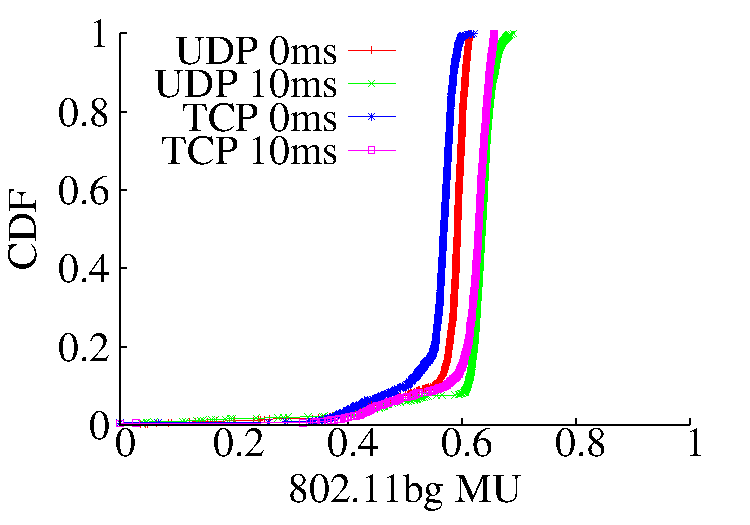
\includegraphics[width=2.5in, angle=0]{./figures/csat_mu_80211bg} 
         \vspace{-0.0cm}
         \caption{Medium Utilization for 802.11 a/g link.}         
        \label{fig:mu_examples_ag}
    \end{subfigure} %

    \begin{subfigure}[b]{\linewidth} \centering 
     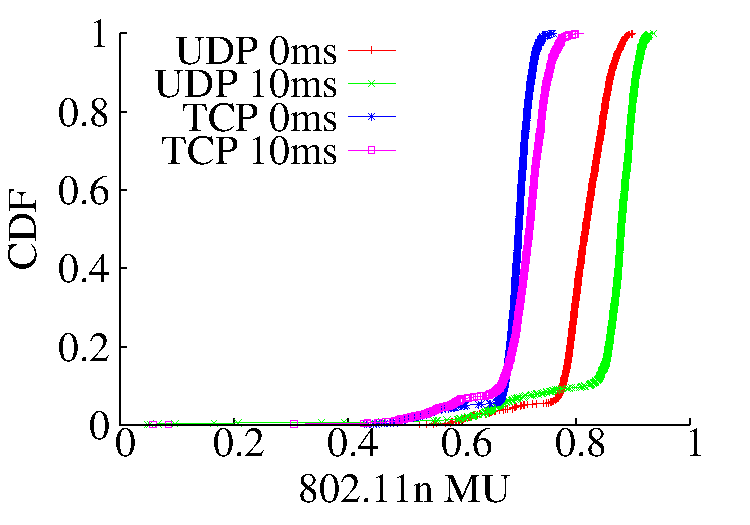
\includegraphics[width=2.5in, angle=0]{./figures/csat_mu_80211n}  
        \vspace{-0.0cm}
        \caption{Medium Utilization for 802.11n link.}
        \label{fig:mu_examples_n}    
    \end{subfigure} 
\caption{Different Medium Utilizations of single Wi-Fi link.}
\label{mu_examples}
\vspace{-0.2cm}
\end{figure}




It is well understood that Wi-Fi's medium utilization depends on a lot of factors, such as PHY data rate, level of packet aggregation, etc. In Figure~\ref{fig:mu_examples_ag}, we plot the MU distributions (\ref{eq:mua}) of a fully backlogged TCP and UDP flow. 
We compare the MU distribution under two different LTE-U duty cycles, 0\% and 50\%, 
and under two different Wi-Fi network types, 802.11a/g and 802.11n.
As we can see, MU varies a lot for a fully backlogged Wi-Fi.
It is therefore very difficult to pick a MU threshold $m$ that works well for all the cases. 
For example, MU goes down to 40\% for 802.11a/g and goes much higher for 802.11n
due to frame aggregation (OpenWRT typically aggregate frames to lengths between 1ms and 4ms).
In Figure~\ref{fig:mu_examples_n}, center and right, we plot the medium utilization for two different duty cycles, 0\% and 50\%. 
As expected, because the Wi-Fi network is fully backlogged, the medium utilization does not change when LTE-U increases the duty cycle. 
We conclude that, in order to avoid starving 802.11n and 802.11a/g links in isolations, 
the MU threshold $m$ has to be under 0.8 and 0.6, respectively. 




\subsection{CSAT and Applications}

The above intuition has been tested so far only in case of fully backlogged flows~\cite{qualcommpresentation}. 
We next look as how the medium utilization changes for various application as we increase the LTE-U duty cycle. 
We present two cases: the good case, where CSAT's design principles hold, and the bad case, where CSAT starves Wi-Fi. 

\noindent{\bf Good case:} 
Figure~\ref{fig:csat_mu_good} shows that for the examples of a rate limited UDP flow (8 Mbps), Youtube (4 Mbps) and Skype (300 kbps), the average medium utilization increases as the LTE-U's duty cycle increases. 
This is inline with the intuition behind CSAT. 
Furthermore, in the UDP and Youtube case, the medium gets saturated and the median medium utilization is 0.65, which is similar to the median medium utilization of a single TCP flow (Figure~\ref{fig:mu_examples_n}).

\begin{figure*}[htb!]
 \centering
    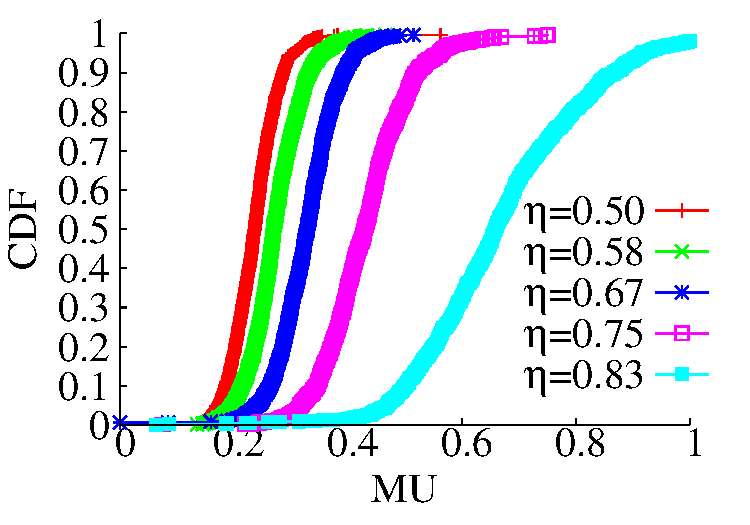
\includegraphics[width=0.3\textwidth]{./figures/csat_mu_udp8mbps}
%    \hspace{-6pt}    
    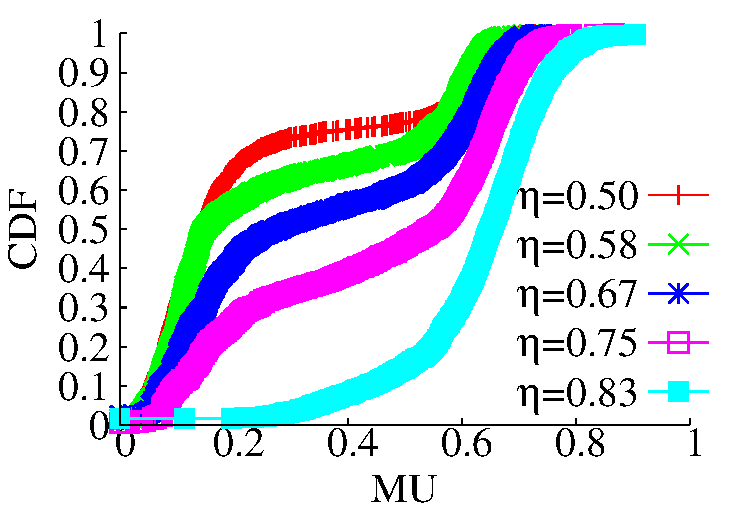
\includegraphics[width=0.3\textwidth]{./figures/youtube_80211bg}
%    \hspace{-18pt}    
    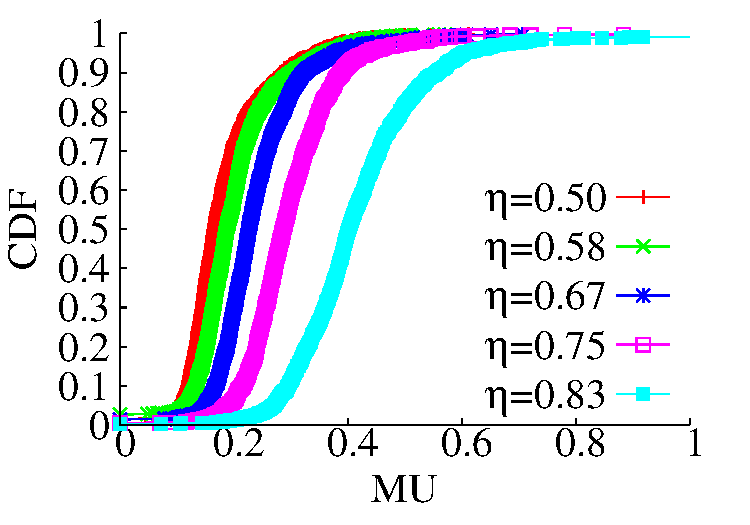
\includegraphics[width=0.3\textwidth]{./figures/skype_80211bg}
%    \hspace{-36pt}    
%    \includegraphics[width=0.98\textwidth]{./figures/good.png}
 \caption{Medium utilization: Good case (left - UDP, 8Mbps; center - Youtube, 4 Mbps; right - Skype, 300 kbps) }
  \label{fig:csat_mu_good}
\end{figure*}



\begin{figure*}[htb!]
 \centering
    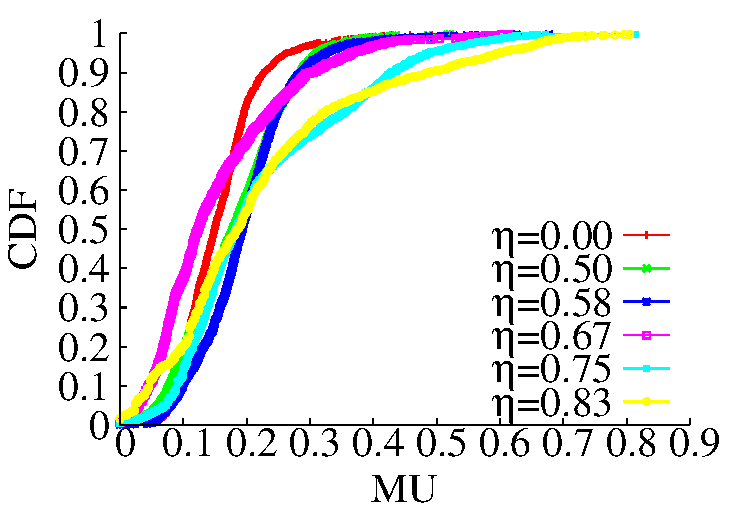
\includegraphics[width=0.3\textwidth]{./figures/bilibili_80211bg}
    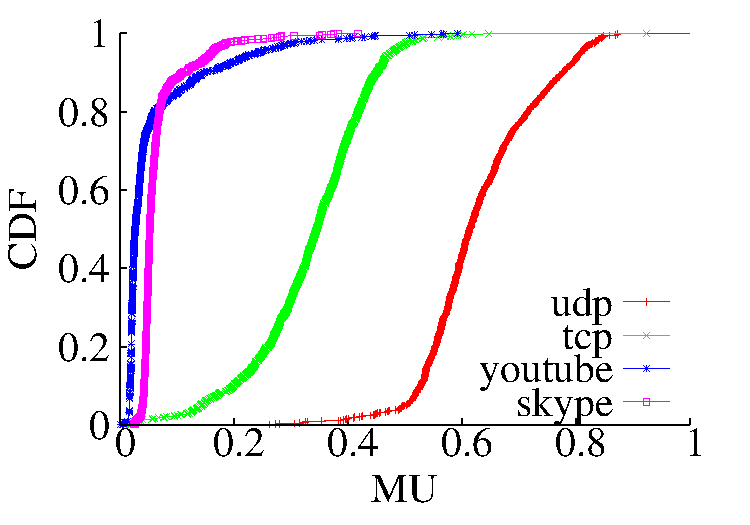
\includegraphics[width=0.3\textwidth]{./figures/hidden_mu_applications}
    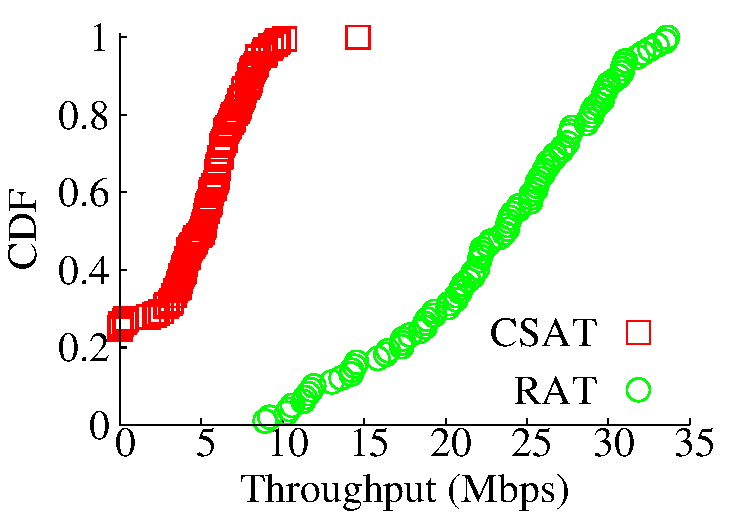
\includegraphics[width=0.3\textwidth]{./figures/hiddencase.pdf}
 \caption{Medium utilization - Bad case: Bilibili traffic, MU in the hidden node case, Wi-Fi throughput for the hidden node case}
  \label{fig:csat_mu_bad}
\vspace{-12pt}
\end{figure*}

\noindent{\bf Bad case:} 
However, this principle does not always work. 
We next consider the case of a Chinese video service Bilibili~\cite{bilibili}, where we again plot the medium utilization as a function of the CSAT duty cycle, in Figure~\ref{fig:csat_mu_bad}, left. 
We see that in this case the basic principle of CSAT does not apply anymore. 
The increase in the duty cycle seems to increase the tail of the medium utilization but not the median. 
Furthermore, we observe that the bilibili video stalls when the medium utilization is 83\%.
In fact, we need to set the CSAT MU threshold very low, around 0.2, to avoid starving the flow. 

We further inspect bilibili traffic and find that it is very bursty. Its bursts last a few seconds and then remains idle for several minutes. This is in contrast with YouTube traffic that is never idle for more than 5 sec. Our measurement interval is 500 ms so we observe that for bilibili traffic the average medium utilization $\overline{MU}$ never gets too high. We conclude that the optimal value of threshold $m$ depends on the application, and it is impossible to find a universal value that makes LTE-U efficient and at the same time avoids starving different applications running over Wi-Fi.

%This illustrate the sensitivity of CSAT to parameters and also shows that a flow can be starved if not properly estimated. 



\begin{figure}[htb!]
\vspace{-12pt}
 \centering
    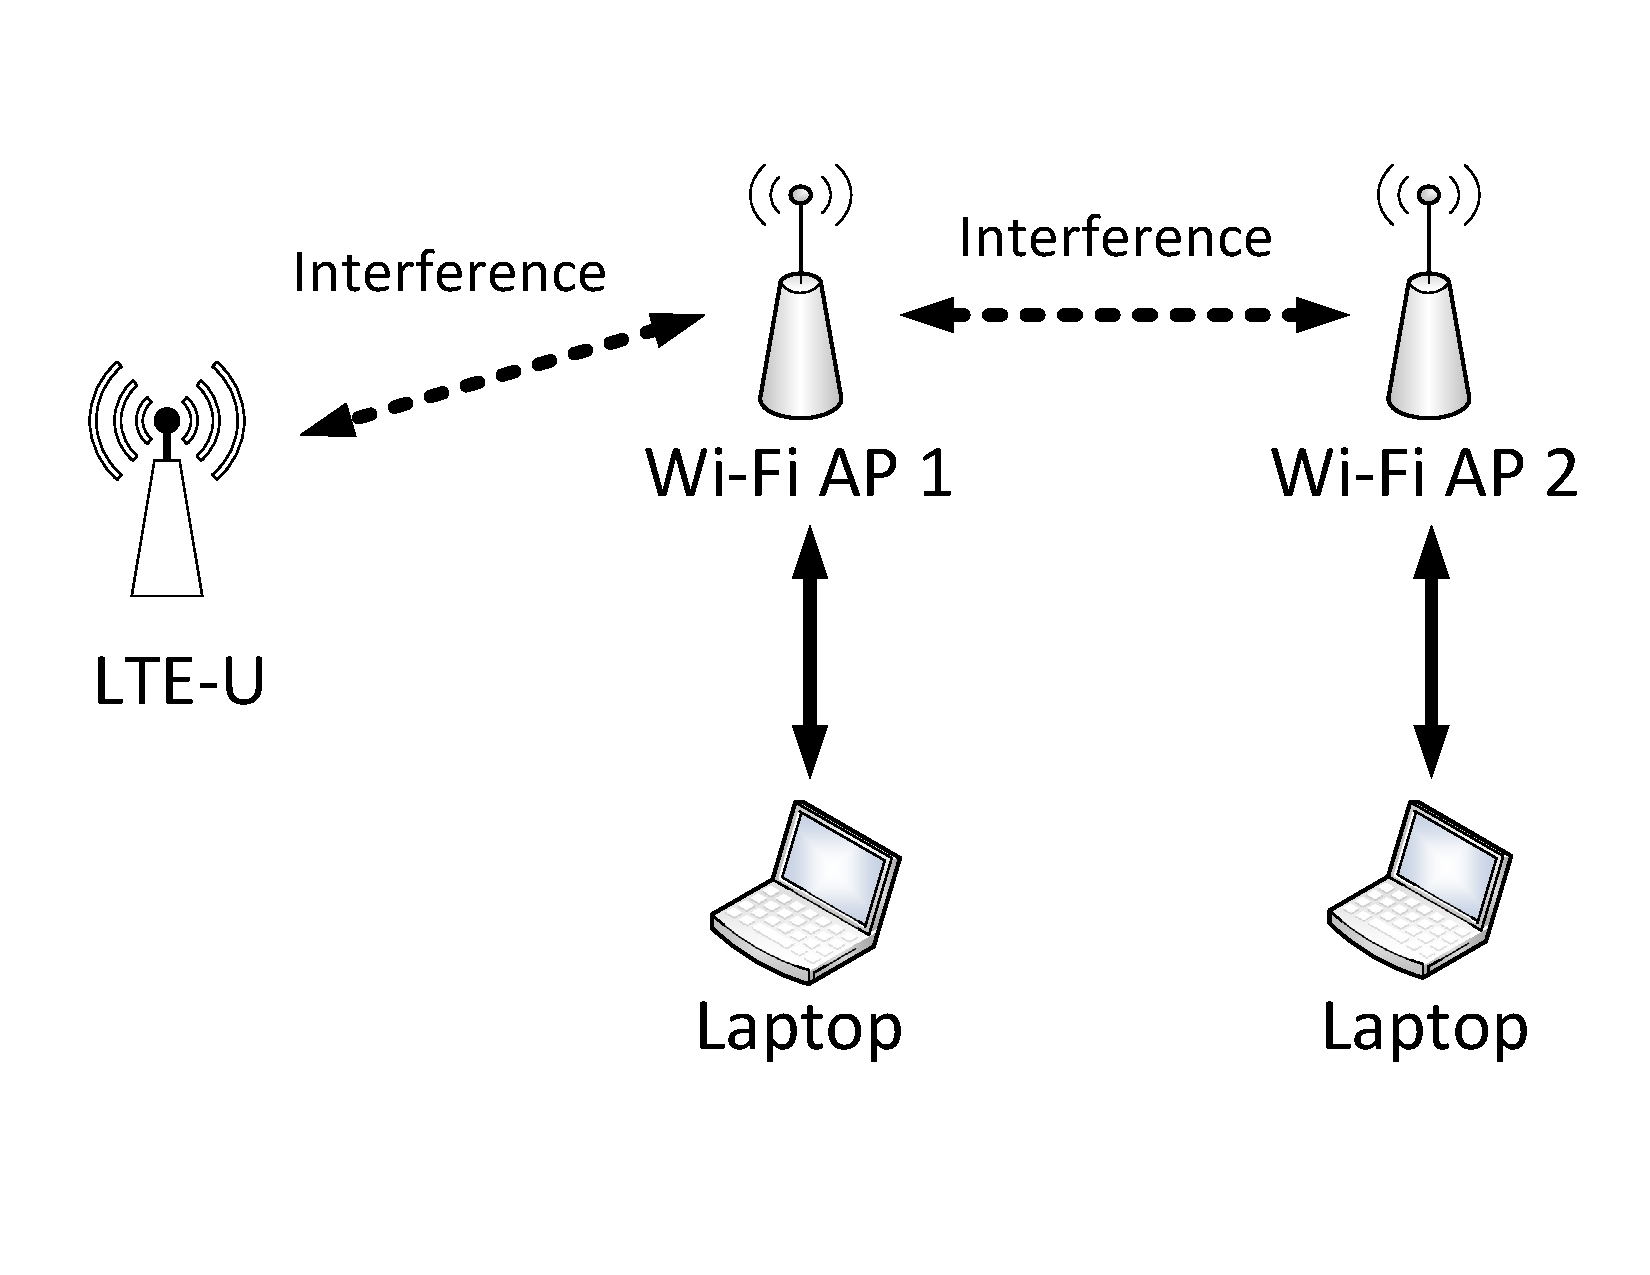
\includegraphics[width=2.4in]{./figures/topology.pdf}
\vspace{-24pt}
 \caption{Topology with a hidden node.}
  \label{fig:csat_hidden}
\vspace{-12pt}
\end{figure}



\subsection{CSAT fails with hidden nodes}

Another reason why CSAT doesn't work is the lack of information about the network. 
Surprisingly, CSAT has so far been tested only in networks where all nodes can sense each other~\cite{qualcommpresentation, google, cablelabs}, which is rarely the case in real-world deployments. 
To illustrate the problem, let us consider a simple network topology illustrated in Figure~\ref{fig:csat_hidden}, with LTE-U node on the left not being able to sense the Wi-Fi 2 AP on the right. 
Even if the Wi-Fi AP 1 in the middle is saturated, its medium utilization will not be high, because it has to share the medium with AP 2. 
The CDF of medium utilization sensed at the LTE-U node is depicted in Figure~\ref{fig:csat_mu_bad}, center. 
Since LTE-U node is not aware of AP 2, and will keep increasing the ON cycle until starving the AP 1. 
The only way this can be alleviated with the existing CSAT algorithm is to reduce the threshold significantly below 40\% which obviously significantly reduces medium utilization.
 
We quantify the effects of CSAT on the hidden node topology in Figure~\ref{fig:csat_mu_bad}, right. In this example we run one TCP flow on each of the Wi-Fi APs. The LTE-U node is fully back-logged, and uses the medium utilization threshold of 40\%. We see that AP 1 is starved 20\% of time, and the rest of the time achieves low throughput, even with the medium utilization threshold as low as 40\%. We further show in Section~\ref{sec:eval} that this issue indeed occurs in real-world networks and that it significantly affects Wi-Fi throughputs. 




%{\bf BR: Here we should try to say why: latency, or something else?}
%{\bf BR: We should plot for this one and the others the actual throughputs for a given sensible MU threshold, to show that it indeed starves.}


